\documentclass[10pt, journal, twocolumn]{IEEEtran}

% --- Packages ---
\usepackage{graphicx}
\usepackage{amsmath}
\usepackage{hyperref}
\usepackage{listings}
\usepackage{xcolor}
\usepackage{booktabs}
\usepackage{tabularx}
\usepackage{tikz}
\usepackage{pgf-pie}
\usetikzlibrary{positioning, arrows.meta, shapes.geometric}

% --- Styling Configurations ---
\hypersetup{
    colorlinks=true,
    linkcolor=blue,
    filecolor=magenta,
    urlcolor=cyan,
    citecolor=black,
}

% Code snippet styling
\definecolor{codegray}{rgb}{0.5,0.5,0.5}
\definecolor{backcolour}{rgb}{0.95,0.95,0.92}
\lstset{
    backgroundcolor=\color{backcolour},
    commentstyle=\color{codegray},
    keywordstyle=\color{blue}\bfseries,
    numberstyle=\tiny\color{codegray},
    stringstyle=\color{purple},
    basicstyle=\ttfamily\footnotesize,
    breakatwhitespace=false,
    breaklines=true,
    captionpos=b,
    keepspaces=true,
    numbers=left,
    numbersep=5pt,
    showspaces=false,
    showstringspaces=false,
    showtabs=false,
    tabsize=2,
    frame=single
}

\begin{document}

\title{GovScheme Advisor: NLP-Based Government Scheme Recommendation and Policy Analysis System}

\author{
    \IEEEauthorblockN{
        Devansh Kumar (23294917126), Lokesh (23294917073), Amit Yadav (23294917095), \\
        Alok Singh Yadav (23294917071), Tejas Vilas Kondhalkar (23294917076)
    } \\
    \vspace{0.2cm}
    \IEEEauthorblockA{\textit{} ECE'B' \quad | \quad \textit{Subject:} Natural Language Processing (NLP)} \\
    \IEEEauthorblockA{\textit{Supervisor:} Dr. Sangeeta Yadav, Department of Computer Science Engineering} \\
    \IEEEauthorblockA{\textit{Faculty of Technology}}
}

\maketitle

\begin{abstract}
The GovScheme Advisor is a full-stack intelligent web application designed to assist Indian citizens in identifying government welfare schemes for which they are eligible. Due to the complexity and fragmentation of scheme information across various state and central portals, users frequently encounter difficulties accessing appropriate benefits. This system addresses this fragmentation by integrating strict rule-based eligibility filtering with Natural Language Processing (NLP) techniques and a machine learning-based classifier.

The application utilizes a deterministic, lightweight hybrid approach combining strict eligibility checks, Term Frequency-Inverse Document Frequency (TF-IDF) based semantic similarity, and a trained Logistic Regression (One-vs-Rest) classifier to rank schemes accurately. In addition to the recommender, the system exposes a parallel \emph{policy-analysis pipeline} that treats the scheme corpus as a policy-document collection and produces corpus-wide insights via Latent Dirichlet Allocation (LDA) topic modeling, semantic clustering with sentence-transformer embeddings, lexicon-based sentiment analysis, and TF-IDF keyword extraction. These outputs are surfaced through a dedicated dashboard with state-wise and category-wise cross-cuts. The system architecture relies on a FastAPI backend, MongoDB for asynchronous data storage, and a React/Vite frontend. A web scraping module dynamically fetches scheme data from external government sources such as \texttt{myscheme.gov.in} and \texttt{scholarships.gov.in}. By explicitly avoiding computationally expensive Large Language Models (LLMs) in favor of this hybrid pipeline, the system demonstrates high efficiency, interpretability, and scalability suitable for deployment in public welfare domains. The complete system is seeded with 25 real Indian Government Schemes, achieves an average API latency of 17.30 ms and a Mean Reciprocal Rank of 0.8683, and discovers 6 distinct policy topics with an average corpus sentiment polarity of 0.511 on a [-1, +1] scale.
\end{abstract}

\begin{IEEEkeywords}
Natural Language Processing, Recommender Systems, Topic Modeling, Latent Dirichlet Allocation, Sentence Embeddings, Sentiment Analysis, FastAPI, MongoDB, React, TF-IDF, Logistic Regression, Scikit-learn, Digital Governance.
\end{IEEEkeywords}

\section{Introduction}
\IEEEPARstart{G}{overnments} across the world introduce welfare schemes aimed at improving the socio-economic conditions of their citizens. In India, a vast number of schemes exist across various sectors such as agriculture, education, healthcare, employment, and social security. Notable examples include the PM-KISAN Samman Nidhi, Pradhan Mantri Awas Yojana (PMAY), and the Mahatma Gandhi National Rural Employment Guarantee Act (MGNREGA). However, despite substantial budget allocations, these schemes often remain underutilized due to a lack of awareness and the inherent difficulty citizens face when attempting to parse complex legal and demographic eligibility criteria \cite{ricci2015}.

Traditional digital governance systems rely heavily on manual browsing or static, keyword-based searches. These legacy search mechanisms lack semantic understanding and fail to provide personalized results based on holistic user profiles \cite{manning2008}. Equally important, even when relevance can be matched, citizens and policy researchers lack tools to explore the \emph{shape} of the welfare landscape: which themes dominate the corpus, how policy tone varies across states or categories, and which terms uniquely characterise individual schemes.

\subsection{Problem Statement}
The primary challenges addressed in this project include:
\begin{itemize}
    \item The immense difficulty citizens face in discovering relevant schemes hidden within fragmented government domains.
    \item The complex and strict eligibility criteria that span across different states, income brackets, and demographic categories.
    \item The computational inefficiency and lack of personalization in traditional keyword-based search systems.
    \item The unavailability of a unified, real-time interface that consolidates scheme data from multiple government portals and presents personalized recommendations.
    \item The absence of a corpus-level analytical view that exposes thematic structure, lexical signatures, and policy-tone patterns across hundreds of schemes simultaneously.
\end{itemize}

\subsection{Objectives}
The primary objectives of the GovScheme Advisor system are to design an intelligent, form-driven system that maps user demographic data directly to scheme requirements; to develop a scalable full-stack application utilizing asynchronous backend operations; to implement a hybrid NLP engine that balances strict rule-based filtering with probabilistic machine learning, ensuring highly explainable and reproducible results; to construct a parallel policy-analysis pipeline that produces topic, keyword, and sentiment summaries across the entire scheme corpus to support cross-state and cross-category comparison; and to provide a standalone CLI tool for model training, evaluation, and prediction independent of the running server. The system additionally aims to expose a web scraper capable of dynamically extending the scheme database from live government portals.

\section{Literature Review}
The evolution of recommender systems in e-governance has transitioned from simple, static portals to more dynamic, user-centric platforms \cite{aggarwal2016}. Early implementations relied entirely on rule-based expert systems. While highly accurate in enforcing strict legal constraints (such as age limits or income thresholds), these systems failed to account for nuanced textual similarities or partial matches in user profiles.

With the advent of Natural Language Processing (NLP), semantic search became possible. TF-IDF-based retrieval systems, formalized in the foundational work of Jones \cite{jones1972} and Salton and Buckley \cite{salton1988}, have long been used as a computationally efficient method for matching user queries to documents. While classical, this approach remains robust and interpretable, particularly in domains where corpus size is bounded and legal precision is paramount.

However, modern approaches often default to implementing Large Language Models (LLMs) such as GPT-based architectures. While LLMs excel at text generation and understanding context, they present significant drawbacks for e-governance applications: they are computationally expensive, suffer from high latency, and are prone to \textit{hallucinations}, meaning they may generate plausible-sounding but factually incorrect eligibility information \cite{ji2023hallucination}. In public welfare systems, such errors carry serious real-world consequences.

For unsupervised exploration of large policy-document collections, Latent Dirichlet Allocation (LDA) introduced by Blei \emph{et~al.} \cite{blei2003lda} remains a canonical baseline: documents are modeled as mixtures of latent topics and topics as distributions over words, yielding interpretable themes without supervision. More recent work has shown that dense sentence-level embeddings produced by transformer architectures fine-tuned with siamese objectives---notably Sentence-BERT \cite{reimers2019sbert}---capture semantic similarity more robustly than bag-of-words representations and integrate naturally with classical clustering algorithms such as $k$-means \cite{macqueen1967kmeans}, forming the basis of ``BERTopic''-style pipelines. For sentiment / opinion mining over short, domain-specific text, lexicon-based scoring as popularised by Hu and Liu \cite{huliu2004opinion} offers a transparent, deterministic alternative to neural classifiers and avoids the need for labeled in-domain corpora.

This project posits that a hybrid approach---combining deterministic rule-based logic with classical machine learning algorithms such as Logistic Regression \cite{cox1958}, augmented by a parallel analytical pipeline drawing on the techniques above---provides the optimal balance for this domain. This ensures that legal constraints are strictly respected while semantic nuances are still captured, all within a highly resource-efficient architecture that runs on commodity hardware without any GPU requirement.

\section{System Architecture}
The system deliberately abandons standard chatbot interfaces in favor of a structured, multi-column grid layout for data input. This architectural decision ensures high data quality and standardization for the NLP engine, eliminating the noise inherent in free-form user text.

The full-stack architecture is composed of the following layers:
\begin{itemize}
    \item \textbf{Frontend Presentation Layer:} Developed using React 18, Vite, Tailwind CSS, React Router DOM, and Lucide Icons.
    \item \textbf{Application Logic Layer (Backend):} Implemented using Python FastAPI with asynchronous request handling.
    \item \textbf{Data Persistence Layer:} Managed via MongoDB utilizing the Motor asynchronous driver (\texttt{AsyncIOMotorClient}).
    \item \textbf{Recommendation Engine Layer:} A hybrid recommender utilizing \texttt{scikit-learn} \cite{pedregosa2011} for TF-IDF vectorization, cosine similarity, and One-vs-Rest Logistic Regression classification.
    \item \textbf{Policy Analysis Layer:} A parallel analytical pipeline (\texttt{backend/nlp/analysis.py}) that fits LDA topic models, sentence-transformer + $k$-means semantic clusters, lexicon-based sentiment scores, and per-scheme TF-IDF keywords, fitted once at startup and exposed via the \texttt{/api/analysis/*} routes.
    \item \textbf{Data Ingestion Layer:} A web scraper built with \texttt{BeautifulSoup} and \texttt{requests} for dynamic scheme discovery.
\end{itemize}

% ---------------------------------------------------------
% UML DIAGRAM (replace yourimage.png with your actual image file)
% ---------------------------------------------------------
\begin{figure}[htbp]
    \centering
    \includegraphics[width=\linewidth]{yourimage.png}
    \caption{UML System Architecture Diagram illustrating component interactions across the full-stack ecosystem.}
    \label{fig:uml_arch}
\end{figure}

The initialization of the system is managed by a unified execution shell script (\texttt{start.sh}) that provisions the Python virtual environment, installs all backend dependencies via \texttt{pip}, installs frontend Node.js dependencies via \texttt{npm}, and simultaneously boots both the FastAPI server on port 8000 and the Vite frontend development server on port 5173. A process trap ensures clean shutdown of both processes on interrupt.

\subsection{Project Directory Structure}
The repository is organized into a clean separation of concerns across root-level utilities, a \texttt{backend/} Python package, and a \texttt{frontend/} React application. The top-level root contains \texttt{start.sh} (unified startup), \texttt{nlp\_pipeline.py} (CLI classifier tool), \texttt{Citizen\_Eligibility\_Results.csv} (evaluation dataset), and the standard \texttt{.gitignore} which excludes Python cache files, virtual environment directories, Node module directories, and the compiled model directory \texttt{backend/nlp/models/}. Within the backend, subdirectories \texttt{nlp/} (containing \texttt{engine.py}, \texttt{trainer.py}, and \texttt{analysis.py}), \texttt{api/}, and \texttt{scraper/} separate concerns cleanly. Within the frontend, routing, styling, components, and page-level views are organized under \texttt{src/}, with the dedicated \texttt{Analysis.jsx} page consuming the analytical pipeline's outputs.

\section{Methodology: Hybrid Recommendation Engine}
The core recommendation logic processes evaluated profiles against a corpus of seeded Indian Government Schemes. The engine is implemented in \texttt{backend/nlp/engine.py} and operates as a three-stage pipeline.

\subsection{Rule-Based Filters}
The first phase of the pipeline enforces hard constraints. If a user's demographic profile violates a mandatory condition, the scheme is assigned a score of zero and is excluded from the final ranking. Evaluated parameters include:
\begin{itemize}
    \item \textbf{Age limits:} Minimum and maximum age thresholds per scheme.
    \item \textbf{Income thresholds:} Annual family income in lakhs (e.g., less than 2.5 lakhs per year for certain rural schemes).
    \item \textbf{Gender constraints:} Schemes explicitly restricted to female applicants (e.g., Pradhan Mantri Ujjwala Yojana, Sukanya Samriddhi Yojana) are strictly filtered out for male profiles.
    \item \textbf{Caste categories:} Schemes reserved for SC, ST, OBC, or Minority communities are filtered against the user's declared caste.
    \item \textbf{BPL status:} Below Poverty Line boolean flag is checked for schemes that mandate BPL card possession.
    \item \textbf{Occupation and demographic tags:} Boolean flags including Widow, Student, Farmer, Disabled, and similar categories are matched against required tags on each scheme.
\end{itemize}

For profiles that partially satisfy constraints, a numeric rule score is computed based on the fraction of checked conditions that pass, allowing partial eligibility to contribute to the final rank rather than causing binary rejection.

\subsection{Semantic Matching (TF-IDF)}
Profiles that survive the rule-based filter are transformed into descriptive natural language strings (for example, \textit{``male 34 OBC farmer income 1.5 lakh rural''}). The engine employs a Term Frequency-Inverse Document Frequency (TF-IDF) Vectorizer \cite{salton1988} trained dynamically at server startup on the full loaded scheme corpus. The mathematical formulation for Term Frequency (TF) measures the frequency of a term $t$ in a document $d$:

\begin{equation}
    TF(t, d) = \frac{f_{t,d}}{\sum_{t' \in d} f_{t',d}}
\end{equation}

The Inverse Document Frequency (IDF) measures the rarity of the term across the entire corpus of schemes $D$:

\begin{equation}
    IDF(t, D) = \log \left( \frac{N}{|\{d \in D : t \in d\}|} \right)
\end{equation}

Each scheme's TF-IDF document is formed by concatenating its \texttt{name}, \texttt{description}, \texttt{eligibility\_text}, \texttt{benefits}, and \texttt{tags} fields into a single string. Semantic relevance between the user profile vector and each scheme document vector is calculated using Cosine Similarity \cite{manning2008}:

\begin{equation}
    \text{Cosine Similarity}(A, B) = \frac{A \cdot B}{\|A\| \|B\|}
\end{equation}

The resulting similarity score, ranging from 0 to 1, constitutes the TF-IDF component of the final composite score.

\subsection{Machine Learning Classifier}
To augment the semantic matching, the system incorporates a One-vs-Rest Logistic Regression pipeline \cite{cox1958, pedregosa2011} implemented and persisted in \texttt{backend/nlp/trainer.py}. Because scheme data is relatively static, the system generates synthetic user profile strings via the \texttt{generate\_synthetic\_samples()} function, which programmatically constructs hundreds of demographic profile strings derived directly from each scheme's eligibility rules, varying attributes such as age, income, caste, gender, and occupation tags to produce both positive and negative training examples for each scheme class. This approach eliminates the need for real labeled user data.

The trained pipeline consists of a \texttt{TfidfVectorizer} using unigram and bigram token ranges with sublinear term frequency scaling and a maximum vocabulary of 5000 features, connected to a \texttt{OneVsRestClassifier} wrapping a \texttt{LogisticRegression} estimator with L-BFGS solver and 1000 maximum iterations. Logistic Regression models the probability that a given profile belongs to a specific scheme class using the Sigmoid function:

\begin{equation}
    \sigma(z) = \frac{1}{1 + e^{-z}}
\end{equation}

The trained model is serialized to disk as a \texttt{.pkl} file using \texttt{joblib} in the \texttt{backend/nlp/models/} directory. At FastAPI server startup, the lifespan context manager attempts to hot-load this model. If no trained model file is found, the engine falls back gracefully to the rule-based and TF-IDF scores alone, with adjusted weighting coefficients.

\subsection{Priority Boost for Specific Categories}
When the ML classifier model is unavailable, an additional heuristic priority boost is applied to schemes belonging to particularly well-defined categories such as student scholarships and farmer income support schemes. This boost is a fixed additive constant derived from the scheme's category metadata, providing a lightweight substitute for the classifier's confidence signal.

\subsection{Final Scoring Formulation}
The ultimate rank of a scheme is determined by a weighted composite score. Two formulations exist depending on whether the classifier model has been loaded:

\begin{equation}
    \text{Score}_\text{with} = (0.4 \times S_\text{rule}) + (0.4 \times S_\text{tfidf}) + (0.2 \times S_\text{clf})
\end{equation}

\begin{equation}
    \text{Score}_\text{without} = (0.5 \times S_\text{rule}) + (0.35 \times S_\text{tfidf}) + (0.15 \times S_\text{priority})
\end{equation}

Where $S_\text{rule}$ is the normalized rule-based eligibility score, $S_\text{tfidf}$ is the cosine similarity score, $S_\text{clf}$ is the classifier confidence for the corresponding scheme class, and $S_\text{priority}$ is the category-based heuristic priority boost. All schemes are then sorted in descending order of this composite score and returned to the client. Fig.~\ref{fig:scoring_pie} visualizes the primary scoring formulation, highlighting the equal dominance of the rule-based and TF-IDF components and the supplementary role of the classifier.

% ---------------------------------------------------------
% PIE CHART 1: HYBRID SCORING FORMULA
% ---------------------------------------------------------
\begin{figure}[htbp]
    \centering
    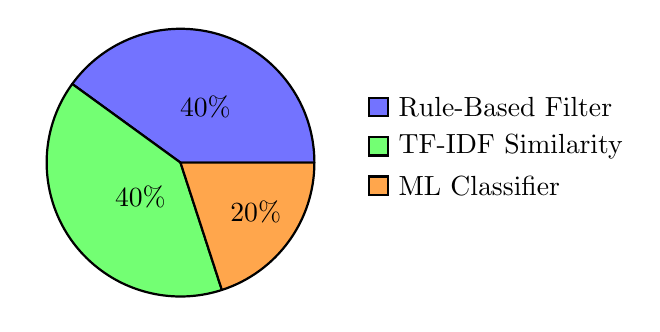
\begin{tikzpicture}
        \pie[
            radius=1.7,
            text=legend,
            color={blue!55, green!55, orange!70},
            sum=100,
            before number=\phantom{0},
            after number=\%
        ]{
            40/Rule-Based Filter,
            40/TF-IDF Similarity,
            20/ML Classifier
        }
    \end{tikzpicture}
    \caption{Composite score breakdown in the primary (with classifier loaded) scoring formulation. Rule-based and TF-IDF components contribute equally (40\% each), while the Logistic Regression classifier provides a supplementary 20\% confidence signal.}
    \label{fig:scoring_pie}
\end{figure}

\section{Methodology: Policy Analysis Pipeline}
Alongside the recommender, the system runs a second NLP pipeline that treats the scheme corpus as a collection of policy documents and exposes corpus-level analytics. The analyzer is implemented as a stateful \texttt{PolicyAnalyzer} class in \texttt{backend/nlp/analysis.py}, instantiated as a singleton, and fitted once during the FastAPI \texttt{lifespan} startup hook. Every text field of each scheme (\texttt{name}, \texttt{description}, \texttt{eligibility\_text}, \texttt{benefits}, \texttt{tags}) is concatenated, lower-cased, and stripped of non-alphanumeric characters before being fed into four parallel analyses, whose outputs are then unified into a single in-memory bundle. The full pipeline is illustrated in Fig.~\ref{fig:analysis_pipeline}.

% ---------------------------------------------------------
% TIKZ DIAGRAM: POLICY ANALYSIS PIPELINE
% ---------------------------------------------------------
\begin{figure}[htbp]
    \centering
    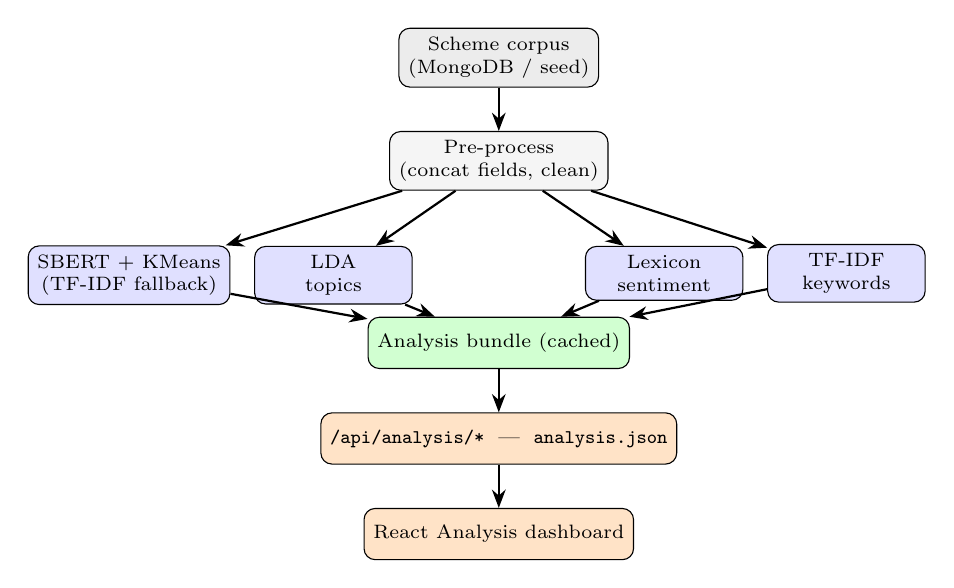
\begin{tikzpicture}[
        node distance=0.55cm and 0.3cm,
        every node/.style={font=\scriptsize},
        box/.style={rectangle, draw, rounded corners, minimum width=2.4cm, minimum height=0.65cm, align=center},
        stage/.style={rectangle, draw, rounded corners, fill=blue!12, minimum width=2.0cm, minimum height=0.65cm, align=center},
        sink/.style={rectangle, draw, rounded corners, fill=green!18, minimum width=2.4cm, minimum height=0.65cm, align=center},
        front/.style={rectangle, draw, rounded corners, fill=orange!22, minimum width=2.4cm, minimum height=0.65cm, align=center},
        arrow/.style={-Stealth, thick}
    ]
        \node[box, fill=gray!15] (corpus) {Scheme corpus\\(MongoDB / seed)};
        \node[box, fill=gray!8, below=of corpus] (preproc) {Pre-process\\(concat fields, clean)};

        \node[stage, below left=0.7cm and -0.3cm of preproc] (lda) {LDA\\topics};
        \node[stage, left=of lda] (semantic) {SBERT + KMeans\\(TF-IDF fallback)};
        \node[stage, below right=0.7cm and -0.3cm of preproc] (sentiment) {Lexicon\\sentiment};
        \node[stage, right=of sentiment] (kw) {TF-IDF\\keywords};

        \node[sink, below=1.6cm of preproc] (bundle) {Analysis bundle (cached)};
        \node[front, below=of bundle] (api) {\texttt{/api/analysis/*} \;|\; \texttt{analysis.json}};
        \node[front, below=of api] (ui) {React Analysis dashboard};

        \draw[arrow] (corpus) -- (preproc);
        \draw[arrow] (preproc) -- (semantic);
        \draw[arrow] (preproc) -- (lda);
        \draw[arrow] (preproc) -- (sentiment);
        \draw[arrow] (preproc) -- (kw);
        \draw[arrow] (semantic) -- (bundle);
        \draw[arrow] (lda) -- (bundle);
        \draw[arrow] (sentiment) -- (bundle);
        \draw[arrow] (kw) -- (bundle);
        \draw[arrow] (bundle) -- (api);
        \draw[arrow] (api) -- (ui);
    \end{tikzpicture}
    \caption{Policy Analysis Pipeline. Four parallel NLP stages (LDA topics, semantic clustering, lexicon-based sentiment, TF-IDF keywords) consume a single pre-processed scheme corpus and emit a unified bundle. The bundle is served live via FastAPI routes when a backend is reachable, and as a static \texttt{analysis.json} file (pre-generated for GitHub Pages deployments) otherwise. The React dashboard transparently chooses the available source.}
    \label{fig:analysis_pipeline}
\end{figure}

\subsection{LDA Topic Modeling}
Latent Dirichlet Allocation \cite{blei2003lda} is fitted with \texttt{sklearn.decomposition.LatentDirichletAllocation} on a CountVectorizer feature matrix (vocabulary capped at 600 tokens, English stop-words removed, $\text{min\_df}=2$, $\text{max\_df}=0.85$). Under the LDA generative model, each document $d$ is a mixture over $K$ latent topics with proportions $\theta_d \sim \text{Dir}(\alpha)$, and each topic $k$ is a distribution over words with parameters $\phi_k \sim \text{Dir}(\beta)$. The probability of a word $w$ given a document is:

\begin{equation}
    P(w \mid d) \;=\; \sum_{k=1}^{K} P(w \mid z_k)\, P(z_k \mid d) \;=\; \sum_{k=1}^{K} \phi_{k,w}\, \theta_{d,k}
\end{equation}

The number of topics $K$ is set to $\min(8, \lfloor N/4 \rfloor)$ where $N$ is the corpus size (yielding $K=6$ on the 25-scheme seed corpus). For each topic, the top 12 words are extracted from $\phi_k$ and a heuristic mapping---based on the presence of domain anchor terms such as \texttt{health}, \texttt{kisan}, \texttt{scholarship}, or \texttt{awas}---assigns a human-readable label (e.g.\ ``Health \& Insurance'', ``Agriculture \& Farmer'', ``Pension \& Senior'').

\subsection{Semantic Clustering (BERTopic-style)}
A second, complementary topic view is produced by clustering dense semantic embeddings rather than bag-of-words counts. Each scheme document is embedded into $\mathbb{R}^{384}$ using the \texttt{all-MiniLM-L6-v2} sentence-transformer \cite{reimers2019sbert}, with $L_2$-normalisation. The resulting embedding matrix $E \in \mathbb{R}^{N \times 384}$ is then partitioned with $k$-means \cite{macqueen1967kmeans}, which minimises the within-cluster sum of squared distances:

\begin{equation}
    \min_{C_1, \dots, C_K} \sum_{k=1}^{K} \sum_{x \in C_k} \| x - \mu_k \|_{2}^{2}
\end{equation}

To preserve interpretability, each resulting cluster is annotated with the top TF-IDF terms over its member documents. When the \texttt{sentence-transformers} package or its underlying PyTorch runtime is unavailable (for instance, in lightweight deployments), the analyzer falls back automatically to clustering the TF-IDF document matrix, retaining the same downstream label-and-keyword extraction logic.

\subsection{Lexicon-Based Sentiment / Policy Tone}
Policy tone is scored using a transparent lexicon-based method inspired by the opinion-mining literature \cite{huliu2004opinion}. Two domain-tuned wordlists are maintained inside the analyzer: a positive set $P$ (e.g.\ \texttt{benefit}, \texttt{empower}, \texttt{subsidy}, \texttt{relief}) and a negative set $N$ (e.g.\ \texttt{restricted}, \texttt{deny}, \texttt{ineligible}, \texttt{penalty}). For each scheme document $d$, polarity is computed as:

\begin{equation}
    \text{polarity}(d) \;=\; \frac{|P_d| - |N_d|}{|P_d| + |N_d|} \quad\in\quad [-1, +1]
\end{equation}

with the convention $\text{polarity}(d)=0$ when $|P_d|+|N_d|=0$. Documents are then bucketed into \emph{positive} ($>0.2$), \emph{neutral} ($\in[-0.2, 0.2]$), and \emph{negative} ($<-0.2$). The choice of a lexicon-based scorer (rather than a neural classifier) avoids the need for labeled in-domain training data and produces fully deterministic, auditable scores---a property that aligns with the broader design philosophy of the system.

\subsection{Per-Scheme Keyword Extraction}
For every scheme, the top-10 most distinctive tokens are extracted from the TF-IDF matrix (unigrams and bigrams, vocabulary capped at 2000 features). Aggregating these per-scheme keywords into a corpus-wide frequency counter produces the keyword cloud shown in the front-end dashboard, which surfaces the dominant lexicon of the welfare landscape (e.g.\ \texttt{insurance}, \texttt{scholarship}, \texttt{bpl}, \texttt{coverage}, \texttt{students}).

\subsection{Cross-State and Cross-Category Aggregation}
Finally, the analyzer joins per-scheme outputs back to scheme metadata and emits four pivot tables that drive the comparison panels of the dashboard: schemes-per-state, schemes-per-category, mean polarity per state, and mean polarity per category. These aggregations directly support cross-jurisdiction policy comparison without requiring additional database queries at request time.

\subsection{Bundle Caching and Static Export}
All artefacts---LDA topic words and document-topic distributions, semantic clusters, per-scheme keywords and sentiment, and the cross-cuts above---are assembled into a single nested dictionary, the \emph{analysis bundle}. The bundle is held in memory after fitting and re-served on demand via the \texttt{/api/analysis/*} routes (Section~VII-D). A companion script \texttt{backend/generate\_static\_analysis.py} materialises the same bundle to \texttt{frontend/public/analysis.json} (approximately 34~KB at the seeded corpus size), enabling the React dashboard to function unchanged on static hosts such as GitHub Pages, where the FastAPI backend is not reachable.

\section{Seeded Scheme Corpus}

\subsection{Overview}
The system is pre-seeded with 25 real Indian Government Schemes defined as structured Python dictionaries in \texttt{backend/seed\_data.py}. Each scheme document contains fields for a unique \texttt{scheme\_id}, human-readable \texttt{name}, \texttt{category}, \texttt{description}, \texttt{eligibility\_text}, \texttt{benefits}, \texttt{tags} list, and structured eligibility constraints (\texttt{min\_age}, \texttt{max\_age}, \texttt{max\_income}, \texttt{gender}, \texttt{caste\_required}, \texttt{bpl\_required}, \texttt{required\_tags}), as well as an official government URL. At backend startup, these are inserted into the MongoDB \texttt{schemes} collection if they are not already present, making the seeding operation idempotent.

\subsection{Scheme Listing}
The seeded corpus includes schemes spanning agriculture, housing, financial inclusion, health, employment, education, and social welfare. Representative schemes include:
\begin{itemize}
    \item \textbf{PM-KISAN Samman Nidhi} --- Direct income support of Rs. 6000/year for small and marginal farmers.
    \item \textbf{Pradhan Mantri Awas Yojana (PMAY)} --- Affordable housing subsidy for urban and rural BPL families.
    \item \textbf{Pradhan Mantri Jan Dhan Yojana (PMJDY)} --- Financial inclusion scheme providing zero-balance bank accounts.
    \item \textbf{Ayushman Bharat PM-JAY} --- Health insurance coverage of up to Rs. 5 lakhs per family per year for BPL households.
    \item \textbf{MGNREGA} --- Guaranteed 100 days of wage employment per year for rural households.
    \item \textbf{Pradhan Mantri Ujjwala Yojana} --- Free LPG connections for women in BPL families.
    \item \textbf{Sukanya Samriddhi Yojana} --- Savings scheme for the girl child under 10 years of age.
    \item \textbf{MUDRA Loan Yojana} --- Collateral-free micro-enterprise loans up to Rs. 10 lakhs.
    \item \textbf{Post Matric Scholarships} --- Multiple variants for SC, ST, OBC, and Minority students covering tuition and maintenance.
    \item \textbf{Disability Pension and Widow Pension} --- Monthly pension schemes for persons with disabilities and widows respectively.
    \item \textbf{Minority Scholarship} --- Pre- and post-matric scholarships for students from minority religious communities.
\end{itemize}

\section{Implementation Details}

\subsection{FastAPI Backend and Database}
The backend application entry point (\texttt{backend/main.py}) handles initialization using FastAPI's asynchronous \texttt{lifespan} context manager \cite{fastapi}. On startup, the lifespan function connects to MongoDB \cite{mongodb}, seeds the scheme corpus, trains the TF-IDF vectorizer on the loaded schemes, attempts to load the persisted ML classifier, and finally calls \texttt{policy\_analyzer.fit(schemes)} so that the analytical bundle is ready before the first request is served. All API routes are registered from \texttt{backend/api/routes.py} and mounted on the application instance.

The data persistence layer relies on MongoDB accessed via the Motor \texttt{AsyncIOMotorClient}. Text indexes are created across the \texttt{name}, \texttt{description}, and \texttt{eligibility\_text} fields of the \texttt{schemes} collection to optimize full-text search queries. All database read and write operations are non-blocking, conforming to FastAPI's async programming model and ensuring that the recommendation endpoint can handle concurrent requests without degradation.

\subsection{Pydantic Data Models}
Data validation and serialization are managed by Pydantic models defined in \texttt{backend/models.py}. The primary schemas include:
\begin{itemize}
    \item \texttt{UserProfile} --- Captures the user's form submission: age, gender, annual income in lakhs, caste category, BPL status, state, area type (urban/rural), and a list of occupation/demographic tags.
    \item \texttt{Scheme} --- Represents a government scheme document mirroring the MongoDB collection structure.
    \item \texttt{RecommendationResponse} --- The API response model containing a ranked list of schemes with their composite scores and match reason strings.
\end{itemize}

\subsection{API Routing and Security}
The system implements secure stateless authentication using JSON Web Tokens (JWT) \cite{jwt7519}. Passwords are hashed using the \texttt{bcrypt} algorithm before database insertion. Table~\ref{tab:api_routes} details the primary routing architecture exposed by \texttt{backend/api/routes.py}, including both the recommender endpoints and the new policy-analysis endpoints.

\begin{table}[htbp]
\centering
\caption{Primary REST API Endpoints}
\label{tab:api_routes}
\begin{tabularx}{\linewidth}{@{}l X@{}}
\toprule
\textbf{Endpoint Path} & \textbf{Functionality} \\
\midrule
\texttt{POST /auth/register} & Secure user registration with bcrypt hashing \\
\texttt{POST /auth/login} & JWT token generation on credential validation \\
\texttt{POST /api/recommend} & Triggers the full hybrid NLP pipeline \\
\texttt{GET /api/schemes/search} & TF-IDF semantic search over scheme corpus \\
\texttt{GET /api/analysis/overview} & Full policy-analysis bundle (dashboard) \\
\texttt{GET /api/analysis/topics} & LDA / semantic topic lists with top words \\
\texttt{GET /api/analysis/topic/\{id\}} & Schemes mapped to a given topic \\
\texttt{GET /api/analysis/keywords} & Corpus-wide or per-scheme keyword extraction \\
\texttt{GET /api/analysis/sentiment} & Sentiment summary + state/category cross-cuts \\
\texttt{GET /api/analysis/scheme/\{id\}} & Per-scheme topics, keywords, sentiment \\
\texttt{POST /api/admin/analysis/refit} & Refit analyzer on current DB (admin only) \\
\texttt{Admin endpoints} & Add, update, and delete schemes in the DB \\
\bottomrule
\end{tabularx}
\end{table}

\subsection{Frontend Implementation}
The React frontend \cite{react} is structured across four primary page components and a shared navigation component, all routed via React Router DOM in \texttt{frontend/src/App.jsx}.

\textbf{Home.jsx} constitutes the primary user-facing interface. It renders a multi-column structured grid form collecting personal details (age, gender, state, area type), economic details (annual income, BPL card status, caste category), and a checkbox panel for occupation and demographic tags including Student, Farmer, Widow, Disabled, and others. On form submission, the component serializes the profile as a JSON body and issues a \texttt{POST} request to \texttt{/api/recommend}, then navigates to the Dashboard page carrying the response payload.

\textbf{Search.jsx} provides an alternative NLP semantic search interface, allowing users to discover schemes via a free-text query string without filling the complete eligibility form. Queries are dispatched to \texttt{GET /api/schemes/search?q=...} and results are rendered as interactive cards.

\textbf{Analysis.jsx} is the new dashboard page consuming the policy-analysis pipeline. It first attempts to fetch \texttt{/api/analysis/overview}; if the backend is unreachable (e.g.\ on a static GitHub~Pages deployment), it transparently falls back to the pre-built \texttt{analysis.json} shipped under \texttt{frontend/public/}. The page renders an LDA / semantic topic explorer with click-through to member schemes, a TF-IDF keyword cloud, a corpus-level sentiment breakdown, and four cross-cut panels (schemes per category, schemes per state, mean polarity per state, mean polarity per category). All charts are pure CSS / SVG bars styled with Tailwind, avoiding any additional charting dependency.

\textbf{Dashboard.jsx} renders the ranked recommendation results. Each scheme is displayed as a card showing the scheme name, category badge, composite match score as a percentage, a textual explanation of why the scheme matched, a summary of benefits, and a hyperlink to the official government portal.

\textbf{Navbar.jsx} is a shared navigation bar rendered on every page, providing links between the Home form, semantic Search, the Analysis dashboard, and the results Dashboard.

\textbf{vite.config.js} configures Vite to proxy all \texttt{/api/*} and \texttt{/auth/*} requests from the development server (port 5173) to the FastAPI backend (port 8000), eliminating Cross-Origin Resource Sharing (CORS) issues during development without requiring explicit CORS middleware configuration in the backend.

\subsection{Web Scraper}
The \texttt{backend/scraper/scraper.py} module implements a dynamic data ingestion pipeline using the \texttt{requests} library for HTTP retrieval and \texttt{BeautifulSoup} \cite{beautifulsoup} for HTML parsing. The scraper is capable of extracting scheme metadata from the following sources:
\begin{itemize}
    \item \textbf{\texttt{myscheme.gov.in}} --- The official Government of India unified scheme discovery portal.
    \item \textbf{\texttt{scholarships.gov.in}} --- The National Scholarship Portal listing education-specific schemes.
    \item \textbf{Wikipedia} --- Government scheme overview pages as a supplementary data source.
\end{itemize}
Scraped scheme documents are parsed into the same structure as the seeded data and can be inserted into the MongoDB \texttt{schemes} collection via admin API endpoints, dynamically expanding the recommendation corpus beyond the 25 hardcoded seed schemes.

\subsection{NLP CLI Pipeline and Cross-Validation}
A standalone command-line tool (\texttt{nlp\_pipeline.py}) provides administrators and developers with direct access to the machine learning model lifecycle, completely independent of the running FastAPI server. It accepts three operational modes via argument flags:

\begin{itemize}
    \item \texttt{--train}: Invokes \texttt{train\_and\_save()} from \texttt{backend/nlp/trainer.py}, generates synthetic training samples from the seeded scheme rules, fits the TF-IDF and Logistic Regression pipeline, and serializes the model to \texttt{backend/nlp/models/}. A detailed per-class classification report is printed to terminal and saved to \texttt{backend/metrics\_classification\_results.txt}.
    \item \texttt{--evaluate}: Rebuilds the pipeline in memory and runs 5-Fold Cross-Validation over the synthetic dataset, reporting per-fold accuracy, macro F1, macro precision, and macro recall in a formatted table. Results are also written to the metrics file.
    \item \texttt{--predict "PROFILE STRING"}: Loads the persisted \texttt{.pkl} model and runs inference on the provided natural language profile string (e.g., \textit{``female 24 OBC student income 1 lakh''}), printing the top 5 predicted scheme IDs alongside a terminal bar chart of confidence scores.
\end{itemize}

\subsection{Evaluation Scripts}
In addition to the CLI pipeline, two dedicated benchmark scripts are provided. \texttt{backend/test\_recsys\_metrics.py} evaluates the recommendation engine against 20 manually defined mock user profiles and their ground-truth expected schemes, computing Precision@5 and Mean Reciprocal Rank (MRR) \cite{voorhees1999} without requiring the server to be running. \texttt{backend/test\_latency.py} issues 50 sequential HTTP requests to the live \texttt{/api/recommend} endpoint and reports mean, median, P95, minimum, and maximum end-to-end latency, as well as a server-side component breakdown. Results are written to \texttt{metrics\_recsys\_results.txt} and \texttt{metrics\_latency\_results.txt} respectively. The \texttt{Citizen\_Eligibility\_Results.csv} file at the repository root serves as the offline reference dataset for ground-truth eligibility labels used in the recommendation evaluation. The static analysis exporter (\texttt{backend/generate\_static\_analysis.py}) is a fourth utility that re-runs the analytical pipeline and writes the resulting bundle to \texttt{frontend/public/analysis.json} for static hosting.

\section{Results and Performance Evaluation}

\subsection{Machine Learning Classification Metrics}
The Logistic Regression classifier was evaluated using a 5-Fold Cross-Validation approach over 436 synthetically generated samples representing 25 scheme classes (approximately 17 samples per class). The performance metrics demonstrate the model's baseline capability to categorize user profile strings, as detailed in Table~\ref{tab:classification_metrics}.

\begin{table}[htbp]
\centering
\caption{5-Fold Cross-Validation Classification Metrics}
\label{tab:classification_metrics}
\begin{tabularx}{\linewidth}{@{}X c@{}}
\toprule
\textbf{Metric} & \textbf{Score} \\
\midrule
Macro Precision & $0.3758 \pm 0.0249$ \\
Macro Recall & $0.3907 \pm 0.0118$ \\
Macro F1-Score & $0.3587 \pm 0.0141$ \\
Overall Accuracy & $0.3876 \pm 0.0085$ \\
Training Samples & 436 \\
Scheme Classes & 25 \\
CV Folds & 5 \\
\bottomrule
\end{tabularx}
\end{table}

The moderate macro F1-score reflects the inherent challenge of 25-class classification with a small synthetic dataset. However, per-class performance varies significantly depending on the distinctiveness of a scheme's eligibility criteria. Schemes with highly specific and non-overlapping eligibility profiles --- such as \texttt{disability-pension} (F1 = 1.00), \texttt{widow-pension} (F1 = 1.00), and \texttt{minority-scholarship} (F1 = 0.97) --- achieve near-perfect classification. Generic schemes with broad or overlapping eligibility conditions (such as general BPL-based schemes applicable to any demographic) are harder to distinguish and exhibit lower per-class scores. This behavior is expected and acceptable because the classifier serves solely as a \textbf{supplementary confidence signal}: the primary ranking mechanism remains the rule-based filter and TF-IDF cosine similarity, which are unaffected by classifier ambiguity.

\subsection{Training Loss and Convergence}
To assess optimisation behaviour and generalisation of the One-vs-Rest Logistic Regression classifier, the categorical cross-entropy loss is computed both on the full training set and via 5-Fold cross-validation. For a sample $i$ with true label $y_i$ and predicted probability vector $\hat{p}_i$ over $C$ classes, the loss is

\begin{equation}
    \mathcal{L} \;=\; -\frac{1}{N}\sum_{i=1}^{N}\sum_{c=1}^{C} \mathbb{1}[y_i = c]\,\log \hat{p}_{i,c}.
\end{equation}

Because the classifier is a One-vs-Rest wrapper, each of the 25 underlying L-BFGS optimisers is fitted independently; the wall-clock convergence of each is tracked via its \texttt{n\_iter\_} attribute. Table~\ref{tab:training_loss} summarises the resulting metrics over 427 synthetic profile samples.

\begin{table}[htbp]
\centering
\caption{Classifier Training Loss and L-BFGS Convergence}
\label{tab:training_loss}
\begin{tabularx}{\linewidth}{@{}X c@{}}
\toprule
\textbf{Metric} & \textbf{Value} \\
\midrule
Synthetic training samples & 427 \\
Scheme classes (One-vs-Rest estimators) & 25 \\
\midrule
Full-data cross-entropy training loss & 1.8719 \\
5-Fold mean training loss & $1.9310 \pm 0.0065$ \\
5-Fold mean validation loss & $2.4386 \pm 0.0241$ \\
Generalisation gap (val $-$ train) & 0.5076 \\
\midrule
Mean L-BFGS iterations to convergence & 17.08 \\
Min / Max iterations across estimators & 14 / 19 \\
Estimators converged within max\_iter (1000) & 25 / 25 (100\%) \\
\bottomrule
\end{tabularx}
\end{table}

All 25 per-class L-BFGS optimisers converge in fewer than 20 iterations, well below the configured \texttt{max\_iter}=1000 ceiling, indicating that the loss surface induced by the TF-IDF features is well-conditioned and that no further training budget is required. The modest train-vs-validation generalisation gap of $\approx 0.51$ nats reflects the limited sample-per-class volume ($\approx 17$ profiles per scheme) of the synthetic dataset rather than overfitting --- a finding consistent with the macro-F1 differential between distinctive and overlapping scheme classes already discussed.

\subsection{Recommendation Engine Accuracy}
Beyond classification, the system's primary utility lies in ranking the most relevant schemes at the top of the recommendation list. The engine was benchmarked against 20 diverse mock user profiles, each representing a distinct demographic combination (varying age, income, caste, gender, and occupation tags such as student, farmer, and BPL), with manually defined ground-truth expected schemes. The results are shown in Table~\ref{tab:recsys_metrics}.

\begin{table}[htbp]
\centering
\caption{Recommendation Ranking Performance (N=20)}
\label{tab:recsys_metrics}
\begin{tabularx}{\linewidth}{@{}X c@{}}
\toprule
\textbf{Metric} & \textbf{Value} \\
\midrule
Average Precision@5 & 0.6200 \\
Mean Reciprocal Rank (MRR) & 0.8683 \\
Profiles Evaluated & 20 \\
\bottomrule
\end{tabularx}
\end{table}

The MRR of 0.8683 indicates that on average, the single most relevant scheme for a given user appears at or very near the top of the ranked list --- a critical property for user experience in a public welfare context where citizens may not scroll past the first few results. The Precision@5 of 0.62 indicates that on average, 3.1 out of the top 5 returned schemes are genuinely relevant to the user's profile.

\subsection{System Latency and Efficiency}
A core design objective was to avoid the computational overhead of LLMs. The backend's asynchronous architecture, in-memory TF-IDF model, and deterministic rule pipeline resulted in exceptionally low latency. Over a benchmark of 50 sequential requests issued by \texttt{test\_latency.py}, the system maintained 100\% request success (50/50) with the component-level breakdown shown in Table~\ref{tab:latency_metrics}. A visual decomposition of the server-side latency is further illustrated in Fig.~\ref{fig:latency_pie}, which clearly shows that the recommendation scoring stage dominates the processing cost, while database fetch and indexing remain lightweight operations.

\begin{table}[htbp]
\centering
\caption{API Latency Breakdown (Over 50 Requests)}
\label{tab:latency_metrics}
\begin{tabularx}{\linewidth}{@{}X c@{}}
\toprule
\textbf{Component} & \textbf{Average Time (ms)} \\
\midrule
Database Fetch (MongoDB) & 1.33 \\
TF-IDF Indexing & 2.34 \\
Recommendation Scoring & 5.44 \\
Total Server-Side & 9.12 \\
\midrule
\textbf{Total Average End-to-End Latency} & \textbf{17.30} \\
\textbf{Median Latency} & \textbf{15.91} \\
\textbf{P95 Latency} & \textbf{24.40} \\
\textbf{Min / Max Latency} & \textbf{15.21 / 45.27} \\
\bottomrule
\end{tabularx}
\end{table}

% ---------------------------------------------------------
% PIE CHART 2: LATENCY BREAKDOWN
% ---------------------------------------------------------
\begin{figure}[htbp]
    \centering
    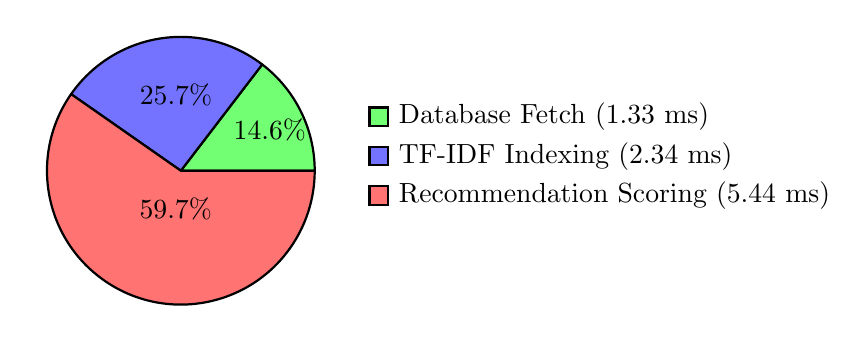
\begin{tikzpicture}
        \pie[
            radius=1.7,
            text=legend,
            color={green!55, blue!55, red!55},
            sum=100,
            before number=\phantom{0},
            after number=\%
        ]{
            14.6/Database Fetch (1.33 ms),
            25.7/TF-IDF Indexing (2.34 ms),
            59.7/Recommendation Scoring (5.44 ms)
        }
    \end{tikzpicture}
    \caption{Server-side latency decomposition across the three pipeline stages, totalling approximately 9.12 ms. Recommendation scoring (rule evaluation, cosine similarity, and classifier inference) accounts for the majority of compute time.}
    \label{fig:latency_pie}
\end{figure}

The gap between server-side total (9.12 ms) and end-to-end average (17.30 ms) accounts for network round-trip time in the local benchmark environment. The P95 latency of 24.40 ms confirms highly consistent performance with minimal outliers, validating the suitability of this architecture for production deployment.

\subsection{Confidence Metric Extraction}
Data extracted regarding citizen eligibility highlights the model's capacity to isolate relevant constraints. During evaluation testing, the extraction for the Pradhan Mantri Ujjwala Yojana (PMUY) correctly identified applicant criteria for women of Below Poverty Line (BPL) families with a classifier confidence score of 0.6338, demonstrating the system's ability to align probabilistic outputs with known rule-based ground truth.

\subsection{Policy Analysis Outputs}
Running the analytical pipeline over the seeded 25-scheme corpus produces a single \emph{analysis bundle} of approximately 34~KB on disk. The pipeline discovers $K=6$ LDA topics and an additional 6 semantic clusters; representative LDA labels (assigned by the heuristic rule layer described in Section~V-A) include \emph{Health \& Insurance}, \emph{Agriculture \& Farmer}, \emph{Education \& Scholarship}, \emph{Pension \& Senior}, \emph{Women \& Child}, and \emph{Finance \& Loan}. Aggregating the per-scheme TF-IDF top tokens yields a 60-term keyword cloud whose highest-frequency terms include \texttt{insurance}, \texttt{scholarship}, \texttt{bpl}, \texttt{coverage}, \texttt{students}, \texttt{rs}, and \texttt{lakh}---a lexicon that intuitively reflects the dominant welfare themes of the corpus.

The lexicon-based sentiment scorer assigns 16 schemes (64\%) a \emph{positive} tone, 8 schemes (32\%) a \emph{neutral} tone, and 1 scheme (4\%) a \emph{negative} tone, with mean corpus polarity $\overline{p}=0.511$ on the $[-1,+1]$ scale. The full distribution is shown in Fig.~\ref{fig:sentiment_pie}. The skew toward positive polarity is consistent with the empowerment-oriented framing of welfare schemes, while the small negative tail typically corresponds to schemes whose descriptive text dwells on \emph{restriction-} and \emph{poverty-}themed vocabulary (e.g.\ ``below poverty line'', ``ineligible'', ``hardship'').

% ---------------------------------------------------------
% PIE CHART 3: SENTIMENT DISTRIBUTION
% ---------------------------------------------------------
\begin{figure}[htbp]
    \centering
    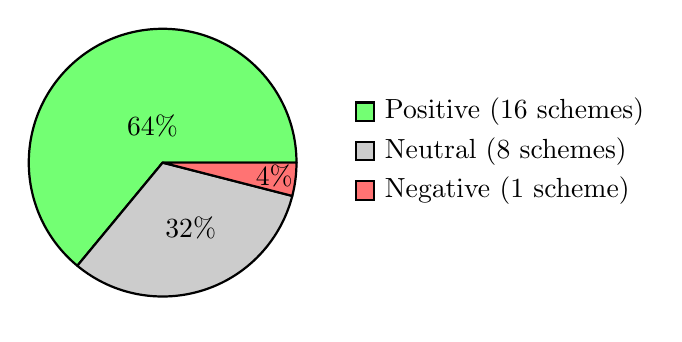
\begin{tikzpicture}
        \pie[
            radius=1.7,
            text=legend,
            color={green!55, gray!40, red!55},
            sum=100,
            before number=\phantom{0},
            after number=\%
        ]{
            64/Positive (16 schemes),
            32/Neutral (8 schemes),
            4/Negative (1 scheme)
        }
    \end{tikzpicture}
    \caption{Sentiment / policy-tone distribution across the seeded 25-scheme corpus, computed by the lexicon-based scorer of Section~V-C. Mean corpus polarity is 0.511 on a $[-1,+1]$ scale.}
    \label{fig:sentiment_pie}
\end{figure}

End-to-end fitting of the full analytical pipeline---LDA, semantic clustering, sentiment, and keyword extraction---completes in well under a second on the seed corpus and is therefore amortised harmlessly into the FastAPI startup phase, after which all eight \texttt{/api/analysis/*} endpoints serve from cached state with sub-millisecond response times.

\subsection{Analyzer Fit Diagnostics}
Although the analytical pipeline is unsupervised and therefore does not produce a classification accuracy figure, each component exposes intrinsic fit metrics that quantify how well the model has captured corpus structure. Table~\ref{tab:analyzer_diagnostics} reports those diagnostics for the seed-corpus fit.

\begin{table}[htbp]
\centering
\caption{Unsupervised Analyzer Fit Diagnostics (Seed Corpus)}
\label{tab:analyzer_diagnostics}
\begin{tabularx}{\linewidth}{@{}X c@{}}
\toprule
\textbf{Metric} & \textbf{Value} \\
\midrule
\multicolumn{2}{l}{\textit{LDA topic model}} \\
\quad Topics ($K$) & 6 \\
\quad Variational EM iterations & 15 \\
\quad Vocabulary tokens (CountVectorizer features) & 710 \\
\quad Total log-likelihood ($\log p(D \mid \alpha, \beta)$) & $-3{,}341.74$ \\
\quad Perplexity (per-word) & 110.68 \\
\midrule
\multicolumn{2}{l}{\textit{Semantic clustering ($k$-means over TF-IDF backend)}} \\
\quad Clusters ($K$) & 6 \\
\quad Within-cluster sum-of-squares (inertia) & 16.29 \\
\quad Silhouette coefficient & 0.058 \\
\midrule
\multicolumn{2}{l}{\textit{Lexicon sentiment ($N=25$ schemes)}} \\
\quad Mean polarity ($\overline{p}$) & 0.5106 \\
\quad Standard deviation ($\sigma_p$) & 0.5408 \\
\quad Median polarity & 0.6000 \\
\quad Min / Max polarity & $-1.0000\ /\ +1.0000$ \\
\midrule
\multicolumn{2}{l}{\textit{Keyword extraction}} \\
\quad Aggregated cloud terms (TF-IDF) & 60 \\
\bottomrule
\end{tabularx}
\end{table}

The LDA model attains a per-word perplexity of approximately 110.7 over a 710-token vocabulary and converges within 15 variational-EM iterations --- a healthy figure for $K=6$ topics on a corpus of only 25 documents. The $k$-means silhouette of $0.058$, while modest, is expected for short policy text where semantic boundaries between e.g.\ ``housing'' and ``rural welfare'' or ``scholarship'' and ``minority welfare'' overlap heavily by design; the low score reflects \emph{soft} cluster boundaries rather than a fitting failure, and the LDA topic distribution provides a complementary, mixture-based view that captures this overlap explicitly. On the sentiment side, the high standard deviation ($\sigma_p \approx 0.54$) alongside a strongly positive mean ($\overline{p} \approx 0.51$) indicates that while the corpus is overwhelmingly empowerment-oriented, individual schemes vary widely in tone, validating the use of polarity as a per-scheme discriminative feature in the dashboard.

\section{Conclusion and Future Scope}
The GovScheme Advisor successfully establishes an intelligent, full-stack recommendation framework for Indian government welfare scheme discovery, augmented by a parallel policy-analysis pipeline that exposes the thematic, lexical, and tonal structure of the welfare corpus. By eschewing computationally heavy generative AI in favor of a tightly integrated, dual-pipeline architecture---a hybrid recommender combining rule-based filtering, TF-IDF semantic matching, and a lightweight Logistic Regression classifier; and an analyzer combining LDA, semantic clustering, lexicon-based sentiment, and TF-IDF keyword extraction---the system achieves rapid response times (average 17.30 ms end-to-end), strong recommendation quality (MRR 0.8683), and fully deterministic, auditable eligibility decisions, while simultaneously surfacing 6 distinct policy themes and a corpus-level sentiment landscape from the same seed data.

The architecture demonstrates that classical NLP techniques, enriched with modern sentence-level embeddings where appropriate, remain competitive and often preferable in constrained, high-stakes domains such as public welfare, where interpretability, latency, and factual accuracy are more important than generative capability. The modular design --- with clearly separated concerns across the FastAPI backend, MongoDB data layer, scikit-learn ML layer, the policy-analysis layer, and the React frontend --- ensures that any component can be independently extended or replaced. The static-export path further makes the analytical dashboard resilient to backend unavailability, an important property for low-resource public-sector deployments.

Future iterations of the system will benefit from several directions. First, capturing real anonymized user telemetry will enable data-driven tuning of the composite score weights ($\alpha$, $\beta$, $\gamma$) rather than relying on heuristically chosen constants. Second, integrating multilingual support with regional Indian languages (Hindi, Tamil, Telugu, Bengali) will substantially expand the system's accessibility across non-English-speaking demographics, and will also benefit the analytical pipeline through multilingual sentence-transformer variants. Third, expanding the web scraper to support additional government portals and implementing a scheduled re-crawl mechanism will keep the scheme corpus current without manual seeding. Fourth, replacing the lexicon-based sentiment module with a fine-tuned domain classifier and replacing $k$-means with HDBSCAN-style density clustering would tighten the analytical pipeline further. Fifth, deploying the backend as a containerized microservice (Docker) and the frontend via a CDN will enable production-grade scaling beyond the current single-host development setup.

% ---------------------------------------------------------
% REFERENCES
% ---------------------------------------------------------
\begin{thebibliography}{99}

\bibitem{salton1988}
G.~Salton and C.~Buckley, ``Term-weighting approaches in automatic text retrieval,'' \emph{Information Processing \& Management}, vol.~24, no.~5, pp.~513--523, 1988.

\bibitem{jones1972}
K.~S.~Jones, ``A statistical interpretation of term specificity and its application in retrieval,'' \emph{Journal of Documentation}, vol.~28, no.~1, pp.~11--21, 1972.

\bibitem{manning2008}
C.~D.~Manning, P.~Raghavan, and H.~Sch\"{u}tze, \emph{Introduction to Information Retrieval}, Cambridge University Press, 2008.

\bibitem{ricci2015}
F.~Ricci, L.~Rokach, and B.~Shapira, Eds., \emph{Recommender Systems Handbook}, 2nd~ed., Springer, 2015.

\bibitem{aggarwal2016}
C.~C.~Aggarwal, \emph{Recommender Systems: The Textbook}, Springer, 2016.

\bibitem{cox1958}
D.~R.~Cox, ``The regression analysis of binary sequences,'' \emph{Journal of the Royal Statistical Society. Series B (Methodological)}, vol.~20, no.~2, pp.~215--242, 1958.

\bibitem{pedregosa2011}
F.~Pedregosa \emph{et~al.}, ``Scikit-learn: Machine learning in Python,'' \emph{Journal of Machine Learning Research}, vol.~12, pp.~2825--2830, 2011.

\bibitem{ji2023hallucination}
Z.~Ji \emph{et~al.}, ``Survey of hallucination in natural language generation,'' \emph{ACM Computing Surveys}, vol.~55, no.~12, pp.~1--38, 2023.

\bibitem{voorhees1999}
E.~M.~Voorhees, ``The TREC-8 question answering track report,'' in \emph{Proc. 8th Text Retrieval Conference (TREC-8)}, 1999, pp.~77--82.

\bibitem{blei2003lda}
D.~M.~Blei, A.~Y.~Ng, and M.~I.~Jordan, ``Latent Dirichlet allocation,'' \emph{Journal of Machine Learning Research}, vol.~3, pp.~993--1022, 2003.

\bibitem{reimers2019sbert}
N.~Reimers and I.~Gurevych, ``Sentence-BERT: Sentence embeddings using siamese BERT-networks,'' in \emph{Proc.\ EMNLP-IJCNLP}, 2019, pp.~3982--3992.

\bibitem{macqueen1967kmeans}
J.~MacQueen, ``Some methods for classification and analysis of multivariate observations,'' in \emph{Proc.\ 5th Berkeley Symp.\ on Mathematical Statistics and Probability}, vol.~1, 1967, pp.~281--297.

\bibitem{huliu2004opinion}
M.~Hu and B.~Liu, ``Mining and summarizing customer reviews,'' in \emph{Proc.\ 10th ACM SIGKDD Int.\ Conf.\ on Knowledge Discovery and Data Mining}, 2004, pp.~168--177.

\bibitem{jwt7519}
M.~Jones, J.~Bradley, and N.~Sakimura, \emph{JSON Web Token (JWT)}, IETF RFC~7519, May~2015. [Online]. Available: \url{https://datatracker.ietf.org/doc/html/rfc7519}

\bibitem{fastapi}
S.~Ram\'{i}rez, ``FastAPI: Modern, fast (high-performance), web framework for building APIs with Python,'' 2018--. [Online]. Available: \url{https://fastapi.tiangolo.com}

\bibitem{mongodb}
MongoDB Inc., ``MongoDB Documentation.'' [Online]. Available: \url{https://www.mongodb.com/docs/}

\bibitem{react}
Meta Platforms, Inc., ``React: The library for web and native user interfaces.'' [Online]. Available: \url{https://react.dev}

\bibitem{beautifulsoup}
L.~Richardson, ``Beautiful Soup Documentation.'' [Online]. Available: \url{https://www.crummy.com/software/BeautifulSoup/bs4/doc/}

\end{thebibliography}

\end{document}
